\documentclass[11pt,a4paper]{article}
\usepackage[margin=23mm]{geometry}
\usepackage[T1]{fontenc}\usepackage{lmodern}
\usepackage{amsmath,amssymb,graphicx,booktabs,array,longtable}
\usepackage{xcolor,fancyhdr}
\usepackage[colorlinks=true,linkcolor=black,citecolor=black,urlcolor=blue!40!black]{hyperref}
\setlength{\headheight}{14pt}\setlength{\parindent}{0pt}\setlength{\parskip}{6pt}
\setlength{\tabcolsep}{4.5pt}\setlength{\emergencystretch}{3em}
\setlength{\LTcapwidth}{.9\linewidth}
\pagestyle{fancy}\fancyhf{}\fancyhead[L]{\small Five-year dementia prediction}\fancyhead[R]{\small BTP report}\fancyfoot[C]{\thepage}
\newcommand{\field}[1]{\texttt{\detokenize{#1}}}
\setcounter{tocdepth}{1}
\begin{document}
\begin{titlepage}\centering\vspace*{8mm}
{\huge\bfseries Predictive Modeling of\par Neurocognitive Disease Progression\par}\vspace{6mm}
{\Large Five-Year Dementia Prediction Using\par Baseline ADNI Tabular Data\par}\vspace{8mm}

\includegraphics[height=38mm]{figures/iit_kharagpur.png}\par\vspace{7mm}
{\large Bachelor's Thesis Project\par}\vspace{3mm}
Thesis submitted to\par
{\Large\bfseries Indian Institute of Technology Kharagpur\par}\vspace{7mm}
In partial fulfillment of the requirements for the award of the degree of\par
{\large B.Tech. in Biotechnology and Biochemical Engineering\par}\vspace{8mm}
Submitted by\par
{\Large\bfseries Ritam Kundu\par}
Roll No.: 23BT10031\par\vfill
Under the guidance of\par
{\large\bfseries Prof. Manjunatha Mahadevappa\par}\vspace{3mm}
Department of Medical Science and Technology\par
IIT Kharagpur\par\vspace{8mm}
\end{titlepage}\setcounter{page}{2}
\thispagestyle{plain}
\phantomsection\addcontentsline{toc}{section}{Candidate's Declaration}
\vspace*{18mm}
\begin{center}{\Large\bfseries Candidate's Declaration}\end{center}
\vspace{8mm}
I hereby declare that this B.Tech. Project-I report titled ``Predictive Modeling of Neurocognitive Disease Progression'' is a record of original work carried out by me as part of a joint project under the guidance of Prof. Manjunatha Mahadevappa, Department of Medical Science and Technology, Indian Institute of Technology Kharagpur, during the period from August 2026 to November 2026, in partial fulfilment of the requirements for the award of the degree of Bachelor of Technology in Biotechnology and Biochemical Engineering.

\vspace{24mm}
\noindent\begin{minipage}[t]{.28\linewidth}
\vspace{0pt}
Kharagpur\par 2026
\end{minipage}\hfill
\begin{minipage}[t]{.64\linewidth}
\vspace{0pt}\raggedleft
\rule{58mm}{.4pt}\par
{\small Candidate signature}\par\smallskip
Ritam Kundu\par Roll No.: 23BT10031
\end{minipage}
\clearpage
\thispagestyle{plain}
\phantomsection\addcontentsline{toc}{section}{Supervisor's Certificate}
\vspace*{18mm}
\begin{center}{\Large\bfseries Supervisor's Certificate}\end{center}
\vspace{8mm}
This is to certify that the B.Tech. Project-I report titled ``Predictive Modeling of Neurocognitive Disease Progression'', submitted by Ritam Kundu (23BT10031) to the Department of Bioscience and Biotechnology in partial fulfilment of the requirements for the award of the degree of Bachelor of Technology in Biotechnology and Biochemical Engineering, is an authentic record of the B.Tech. Project-I work carried out by the candidate under my supervision and guidance. The report has fulfilled all the requirements as per the regulations of the Institute.

\vspace{24mm}
\noindent\begin{minipage}[t]{.28\linewidth}
\vspace{0pt}
Kharagpur\par 2026
\end{minipage}\hfill
\begin{minipage}[t]{.64\linewidth}
\vspace{0pt}\raggedleft
\rule{58mm}{.4pt}\par
{\small Supervisor signature}\par\smallskip
Prof. Manjunatha Mahadevappa\par Department of Medical Science and Technology\par Indian Institute of Technology Kharagpur
\end{minipage}
\clearpage
\section*{Abstract}\addcontentsline{toc}{section}{Abstract}
In this project, we developed a machine-learning pipeline to estimate whether an ADNI participant with an eligible baseline record will receive a dementia diagnosis within the following five years. The analysis uses structured demographic, genetic, cognitive, medical-history and biomarker information. The prediction target is observed all-cause dementia based on the harmonized DXSUM diagnosis; it is not limited to dementia caused specifically by Alzheimer's disease.

We used 17 local source tables and a feature audit that identified 67 candidate variables for data preparation. Seven plasma candidates were deferred because their measurements could not be reliably established as available before the baseline date. The remaining 60 candidate predictors were prepared through two feature-extraction handoffs and merged after checks for participant identity, duplicate rows, variable overlap and measurement timing. Imaging is represented by numeric measurements derived from scans. Raw MRI and PET files are not model inputs.

Among 2,155 baseline participants, 1,056 had sufficiently clear five-year outcomes: 324 were observed dementia converters and 732 were observed non-converters. Participants with baseline dementia, insufficient follow-up or ambiguous diagnosis records were not used for binary model training.

The labeled cohort was divided into development (633 participants), calibration (211) and final validation (212) sets. This report documents the ECog, NEUROBAT and MEDHIST handoff and the CatBoost and Random Forest comparisons. The strongest of these tree candidates was core-panel CatBoost, with mean development F1 of 0.8505. The tree comparisons were development experiments. The shared frozen project predictor achieved 89.62\% accuracy, 83.08\% precision, 83.08\% recall, 92.52\% specificity, F1 of 0.8308 and ROC AUC of 0.9667 on final validation.

These results show that a carefully prepared baseline tabular dataset can support useful discrimination in the selected ADNI cohort. However, the analysis excludes participants with incomplete five-year observation and has limited external validation. It should be considered a reproducible research result, not a clinically validated risk calculator.

\clearpage\tableofcontents\clearpage
\section{Introduction}
Alzheimer's disease (AD) is a progressive neurodegenerative condition and an important cause of dementia. Cognitive decline can develop gradually, and individuals with similar baseline clinical profiles may follow different disease trajectories. For this reason, it is useful to study not only whether a person currently has cognitive impairment, but also whether the available baseline information can help identify people who may develop dementia during a future period.

The Alzheimer's Disease Neuroimaging Initiative (ADNI) is a longitudinal research study that collects clinical, cognitive, imaging, genetic and biological measurements from participants across multiple study phases. These data allow researchers to investigate changes associated with normal aging, mild cognitive impairment and Alzheimer's disease over time. The project described in this report uses a local ADNI data snapshot to build a five-year prediction pipeline.

The central idea is to use only information available at the participant's original baseline visit. This is important because information collected after baseline may already reflect disease progression. Using such future information would make the model appear more accurate than it would be in a real prediction setting. This problem is known as temporal data leakage.

The project is a prognosis task rather than a current-diagnosis task. Participants who already had dementia at baseline were excluded. The outcome was defined from the harmonized DXSUM diagnosis trajectory and represents any observed dementia diagnosis within five calendar years after baseline. Therefore, the task is not restricted to Alzheimer's disease as the cause of dementia.

\section{Objectives}
\begin{itemize}
\item To study the different types of data available in the ADNI database and understand how these data are collected during longitudinal visits.

\item To prepare a participant-level baseline dataset by combining relevant demographic, genetic, cognitive, medical-history and biomarker information.

\item To construct a reliable five-year dementia outcome using follow-up diagnosis records while excluding baseline dementia and uncertain outcomes.

\item To compare multiple machine-learning algorithms and select a suitable model for the available tabular dataset.

\end{itemize}
\section{Literature Review}
Pathak et al. (2026) study Alzheimer's disease classification from resting-state fMRI \cite{pathak}. Their work illustrates a separate ADNI use case: learning from functional connectivity to identify current disease status. This project instead forecasts observed dementia conversion from baseline tabular measurements.

\subsection{Earlier approaches to functional connectivity}
Resting-state fMRI measures changes in the blood-oxygen-level-dependent (BOLD) signal while a participant is resting. A common approach is to extract an average time series from each brain region and calculate pairwise correlations between regions. These correlations form a functional connectivity (FC) matrix. Earlier studies used selected connectivity measures with conventional classifiers such as support vector machines. Although useful, handcrafted summaries may not fully capture complex and non-linear relationships between widely separated brain regions.

Deep-learning approaches have also been explored. Convolutional neural networks can learn representations from connectivity matrices or fMRI data, but local convolution operations may be less suitable for relationships distributed across the whole brain.

\subsection{Attention-based approach in the paper}
Pathak et al. propose a Transformer-inspired self-attention model. Instead of treating each brain region only as part of a fixed connectivity image, the model treats each region of interest (ROI) as a token. A learnable linear layer maps this connectivity profile into an embedding. Multi-head self-attention then allows each ROI representation to use information from other functionally related regions.

The attention outputs are combined using global mean pooling. The resulting visit-level representation is passed to a fully connected classifier containing layer normalization, linear layers, ReLU activation and dropout. A sigmoid function converts the final score into a probability of the Alzheimer's disease class. The model is trained using the AdamW optimizer and a class-weighted binary cross-entropy loss.

\subsection{Dataset and reported findings of the paper}
The paper uses data from ADNI-GO, ADNI-2 and ADNI-3. Its final cohort contains 60 participants: 30 diagnosed with Alzheimer's disease and 30 cognitively normal controls. Each participant contributes two visits approximately one year apart, giving 120 visit-level samples. Each visit includes a structural T1-weighted MRI scan and an rs-fMRI scan. The structural scan supports anatomical alignment, while the classifier operates on rs-fMRI functional connectivity.

The rs-fMRI preprocessing described in the paper includes slice-timing correction, head-motion correction using FSL MCFLIRT, registration to the participant's T1-weighted image, normalization to MNI152 standard space, spatial smoothing with a 4--5 mm Gaussian kernel, and temporal filtering between 0.01 and 0.1 Hz. The brain is divided into 69 cortical and subcortical ROIs using the Harvard--Oxford atlas. Mean BOLD time series are extracted and pairwise Pearson correlations are used to form the FC matrix.

\begingroup\small\renewcommand{\arraystretch}{1.16}
\begin{longtable}{@{}>{\raggedright\arraybackslash}p{0.28\linewidth}>{\raggedright\arraybackslash}p{0.68\linewidth}@{}}
\caption{Main components of the attention-based rs-fMRI model reported by Pathak et al. \cite{pathak}}\\
\toprule \textbf{Item} & \textbf{Description}\\\midrule\endfirsthead
\toprule \textbf{Item} & \textbf{Description}\\\midrule\endhead
\midrule\endfoot\bottomrule\endlastfoot
Input to attention model & 69 \ensuremath{\times} 69 functional connectivity matrix for each visit\\
ROI representation & Each row is projected into a 128-dimensional embedding\\
Attention & Multi-head self-attention with 4 attention heads\\
Pooling and classifier & Global mean pooling followed by a fully connected classifier\\
Training settings & AdamW, learning rate $1\times 10^{-4}$, batch size 8, 40 epochs, dropout 0.3\\
\end{longtable}\endgroup
The paper motivates the use of brain measurements and subject-level evaluation. Its attention architecture, rs-fMRI processing and present-diagnosis target are distinct from the baseline tabular prognosis implemented here.

\section{Types of Data in ADNI and Their Collection}
ADNI is a multi-site, longitudinal research study. Participants are assessed according to study-phase protocols and visit schedules. Much of the information is collected during in-person clinical visits, while some follow-up information may be collected by telephone, online assessment or remote questionnaires. The exact set of procedures depends on the ADNI phase, participant group and scheduled visit; therefore, not every participant has every type of data \cite{collection}.

\subsection{Major data categories}
\begingroup\small\renewcommand{\arraystretch}{1.16}
\begin{longtable}{@{}>{\raggedright\arraybackslash}p{0.2\linewidth}>{\raggedright\arraybackslash}p{0.3\linewidth}>{\raggedright\arraybackslash}p{0.45\linewidth}@{}}
\caption{Major ADNI data categories and their typical collection routes \cite{collection,docs}}\\
\toprule \textbf{Data type} & \textbf{Examples} & \textbf{How the data are collected}\\\midrule\endfirsthead
\toprule \textbf{Data type} & \textbf{Examples} & \textbf{How the data are collected}\\\midrule\endhead
\midrule\endfoot\bottomrule\endlastfoot
Demographic and subject information & Age, sex, education, race/ethnicity, marital status, family history, medications & Recorded during screening and clinical visits through participant interviews, study forms and questionnaires.\\
Clinical and diagnostic data & Clinical diagnosis, medical history, physical and neurological examination, functional status & Collected by trained clinical staff using standardized assessments and protocol-defined diagnostic procedures.\\
Cognitive and neuropsychological data & MMSE, MoCA, ADAS-Cog, CDR, RAVLT, memory, attention, language and executive-function tests & Participants complete structured cognitive tests administered by trained assessors; study partners may provide additional functional assessments.\\
Structural MRI & T1-weighted MRI, T2, FLAIR and derived brain-region volumes & MRI scans are acquired at imaging centres using phase-specific scanner protocols; images undergo quality checks and processing.\\
Functional MRI and diffusion imaging & Resting-state fMRI, diffusion tensor imaging (DTI) & MRI sequences capture BOLD signal changes or water-diffusion information. These data require dedicated preprocessing and quality control.\\
PET imaging & FDG-PET, amyloid PET and tau PET & Participants undergo PET scans using an appropriate tracer. Images are processed to derive measures of brain metabolism or molecular pathology.\\
Biofluid biomarkers & CSF amyloid-\ensuremath{\beta} and tau; blood/plasma biomarkers such as p-tau, NfL and GFAP; urine measures & Blood and urine are collected by sample procedures. CSF is generally obtained through lumbar puncture. Samples are processed, stored and analysed by designated laboratories.\\
Genetic and other omics data & APOE genotype, GWAS, sequencing, methylation, RNA and other molecular profiles & Usually derived from collected biological samples such as blood. DNA/RNA or other molecular material is processed and analysed using laboratory assays.\\
Digital and remote assessments & Online cognitive tests, digital questionnaires and telephone follow-ups & Collected through approved remote instruments, online platforms, telephone calls or mailed questionnaires, depending on study phase.\\
Neuropathology & Brain tissue measurements and digitized slide images & Available for participants who consent to brain donation; tissue is examined after death through neuropathological procedures.\\
\end{longtable}\endgroup
\subsection{How collection is standardized}
ADNI uses common protocols so that measurements from different clinical sites can be compared across participants and over time. Each participant is assigned a coded identifier, and records are linked to visits. The visit schedule determines which clinical tests, scans or biospecimens are expected at that time. This creates repeated measurements that can be used to study longitudinal change.

Clinical assessments and questionnaires are commonly administered by trained staff. Some instruments are first recorded on paper forms and later entered into an electronic data-capture system. Imaging files are processed and checked for quality before being made available. Biofluid samples are placed in labelled vials, shipped to designated laboratories, and analysed or stored. Because each modality follows its own path from collection to the final database, the available date and format of a variable should be checked before it is used in a prediction model \cite{collection}.

A practical point is that ADNI data are not simply one spreadsheet. The database contains multiple tables and image collections, linked by participant identifiers and visit codes. One participant may have several rows in a clinical table and several imaging or laboratory records. A correct analysis must therefore identify the intended visit, preserve participant identity and avoid creating duplicate participant records when tables are merged.

\subsection{Main ADNI tables used}
\begingroup\small\renewcommand{\arraystretch}{1.16}
\begin{longtable}{@{}>{\raggedright\arraybackslash}p{0.29\linewidth}>{\raggedright\arraybackslash}p{0.66\linewidth}@{}}
\caption{Important local source tables and their role in the project}\\
\toprule \textbf{Source table/file} & \textbf{Role in the project data review}\\\midrule\endfirsthead
\toprule \textbf{Source table/file} & \textbf{Role in the project data review}\\\midrule\endhead
\midrule\endfoot\bottomrule\endlastfoot
ADNIMERGE & Main longitudinal merged table; used as the primary source for baseline demographics, cognitive scores and numerical imaging/biomarker composites.\\
DXSUM & Contains diagnosis information across visits; used to construct the five-year outcome.\\
MEDHIST & Contains medical-history records; used to create selected pre-baseline history flags.\\
NEUROBAT & Contains neuropsychological test measurements; used for supplementary baseline/screening candidates.\\
UPENN plasma & Contains plasma biomarker records; reviewed, but plasma candidates were deferred from the primary model because pre-baseline coverage was limited.\\
TADPOLE D1/D2 and dictionary & Used as reference material for baseline selection, candidate variables and variable descriptions; not treated as an independent test cohort.\\
dfMri / dfMri D12 & MRI extraction tables reviewed during the inventory; redundant measurements were not added again to the primary feature matrix.\\
\end{longtable}\endgroup
\section{Data Used in This Project}
The current project uses structured baseline information rather than raw medical images. The starting participant pool contains 2,155 unique original-baseline participants. The data preparation process identified 67 candidate variables from the local source inventory. Seven plasma candidates were deferred because only limited baseline-overlapping, pre-index samples were available in the initial feasibility review. This left 60 assigned source predictors for the prepared feature matrix.

\subsection{Feature groups}
\begingroup\small\renewcommand{\arraystretch}{1.16}
\begin{longtable}{@{}>{\raggedright\arraybackslash}p{0.33\linewidth}>{\raggedright\arraybackslash}p{0.62\linewidth}@{}}
\caption{Feature families in the candidate specification}\\
\toprule \textbf{Feature group} & \textbf{Examples used or considered}\\\midrule\endfirsthead
\toprule \textbf{Feature group} & \textbf{Examples used or considered}\\\midrule\endhead
\midrule\endfoot\bottomrule\endlastfoot
Demographics and genetics & Age, sex, education and APOE4 allele count.\\
Core cognitive assessments & CDRSB, ADAS11, ADAS13, MMSE, RAVLT measures, FAQ and MoCA.\\
CSF biomarkers & Baseline amyloid-\ensuremath{\beta} (ABETA), total tau (TAU) and phosphorylated tau (PTAU).\\
Imaging-derived numerical measures & Hippocampal, ventricular, whole-brain, entorhinal, fusiform and middle-temporal volumes; intracranial volume; FDG-PET composite.\\
Medical history & Selected pre-index cardiovascular, endocrine and smoking history flags, with additional history candidates in the expanded panel.\\
Supplementary cognition and self-report & ECog participant/study-partner scores and selected NEUROBAT test scores.\\
\end{longtable}\endgroup
\subsection{Final model feature panel}
Three panels were compared: clinical (14 source variables), core (28 source variables), and expanded (60 assigned non-plasma source variables). The project's frozen predictor uses the 28-variable core panel. It adds CSF biomarkers, imaging-derived measures and three medical-history flags to the clinical panel.

\begingroup\small\renewcommand{\arraystretch}{1.16}
\begin{longtable}{@{}>{\raggedright\arraybackslash}p{0.3\linewidth}>{\raggedright\arraybackslash}p{0.15\linewidth}>{\raggedright\arraybackslash}p{0.48\linewidth}@{}}
\caption{Core feature panel used by the final project predictor}\\
\toprule \textbf{Core panel component} & \textbf{Number of source variables} & \textbf{Examples}\\\midrule\endfirsthead
\toprule \textbf{Core panel component} & \textbf{Number of source variables} & \textbf{Examples}\\\midrule\endhead
\midrule\endfoot\bottomrule\endlastfoot
Demographic/genetic and cognition & 14 & Age, sex, education, APOE4 and 10 core cognitive measures\\
CSF biomarkers & 3 & ABETA, TAU and PTAU\\
Structural MRI-derived measures & 7 & Hippocampus, ventricles, whole brain, entorhinal, fusiform, middle temporal and ICV\\
FDG-PET composite & 1 & Baseline FDG measure\\
Medical-history flags & 3 & Cardiovascular, endocrine and smoking history flags\\
Total & 28 & Selected core source features\\
\end{longtable}\endgroup
Although some predictors originate from MRI or PET examinations, they are numerical summaries already provided in the ADNI tables. The project does not train a neural network on raw MRI/PET images and does not use the raw rs-fMRI scans from the attached literature paper.

\clearpage
\section{Methodology and Model}
\subsection{Overall workflow}
\par\medskip\noindent\begin{minipage}{\linewidth}\centering
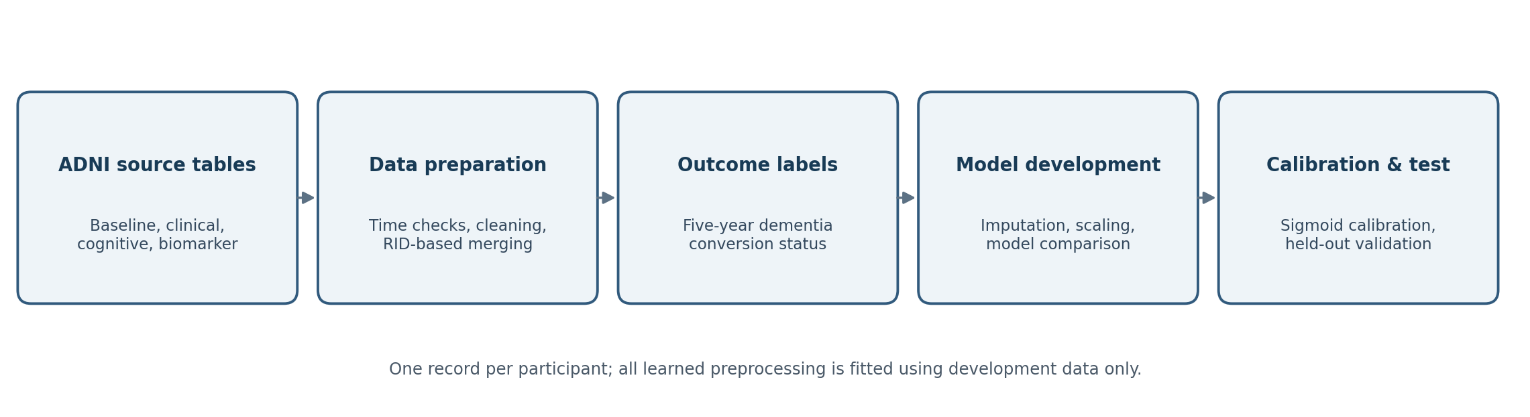
\includegraphics[width=.98\linewidth,height=.63\textheight,keepaspectratio]{figures/workflow.png}
\par\smallskip\refstepcounter{figure}\small Figure \thefigure: Overview of the baseline tabular prediction workflow.\end{minipage}\par\medskip
\subsection{Construction of the five-year outcome}
For each participant, the original baseline date is treated as the prediction date. A five-calendar-year horizon is calculated from this date. The harmonized diagnosis values in DXSUM are then ordered by their assessment dates. Diagnosis code 1 represents cognitively unimpaired status, code 2 represents mild cognitive impairment, and code 3 represents dementia.

Positive outcome (converter): a dementia diagnosis is recorded after baseline and on or before the five-year anniversary.

Negative outcome (observed non-converter): no dementia diagnosis is recorded within the five-year window and there is a valid diagnosis observation at or beyond the five-year horizon.

Unknown outcome: there is not enough follow-up to establish either condition, or the diagnosis records are ambiguous. Such participants are not treated as negative cases.

Participants with dementia at baseline, missing or unrecognized baseline diagnosis, or undated dementia records were excluded. An event recorded exactly on the five-year anniversary counts as positive. A later diagnosis reversion does not erase an earlier dementia event.

\begingroup\small\renewcommand{\arraystretch}{1.16}
\begin{longtable}{@{}>{\raggedright\arraybackslash}p{0.75\linewidth}>{\raggedright\arraybackslash}p{0.2\linewidth}@{}}
\caption{Participant counts after outcome construction and eligibility checks}\\
\toprule \textbf{Outcome disposition} & \textbf{Participants}\\\midrule\endfirsthead
\toprule \textbf{Outcome disposition} & \textbf{Participants}\\\midrule\endhead
\midrule\endfoot\bottomrule\endlastfoot
Observed five-year non-converters & 732\\
Incident dementia within five years & 324\\
Insufficient follow-up & 698\\
Baseline dementia & 367\\
Unknown baseline diagnosis & 23\\
Undated dementia record & 8\\
Conflicting same-day diagnoses & 2\\
Dementia at or before baseline & 1\\
Total original-baseline participants & 2,155\\
\end{longtable}\endgroup
\subsection{Data cleaning and feature preparation}
The project combines two feature-extraction handoffs. Each handoff retains the participant roster identifier (RID), and the merge checks that there is one row per RID, that both handoffs contain the same participant set, and that no predictor names overlap. The merge is validated as one-to-one. Participant identifiers, visit dates and diagnosis fields are retained as audit metadata and are not used as model predictors.

\subsubsection*{Individual report focus: ECog, NEUROBAT and MEDHIST handoff}
The two handoffs were prepared as part of a joint project. This report documents the 31-field supplementary block: 14 baseline Everyday Cognition (ECog) scores from ADNIMERGE, ten selected NEUROBAT measures and seven MEDHIST flags. Its keys are checked against the same 2,155 baseline participants before joining the handoffs.

NEUROBAT rows were matched using actual assessment dates and screening or baseline visit codes. Eligible visits had to fall at the index date or within the previous 90 days. Screening was preferred for Logical Memory; baseline was preferred for other measures. Within the preferred visit group, the most recent eligible assessment was chosen. Conflicting results at the same priority and date were treated as missing rather than resolved arbitrarily. The audit recorded between 30 and 120 changed values per test column relative to the supplied handoff.

MEDHIST rows were filtered to dates at or before index. A condition became 1 if any eligible record documented it and 0 if eligible records documented absence without a positive record. Unavailable history remained missing. This corrected the earlier zero coding for 417 participants without usable pre-baseline history. This distinction matters because lack of a history record does not imply lack of a condition.

The normalization focus here is harmonizing visit timing, numeric test-score fields and binary history coding. Values were left in the source test units and history retained its 0/1/missing representation in the prepared matrix. No independent full-cohort scaler was applied to this handoff. After joining, numerical transformations were learned on each training fold; this preserves the common validation boundary and retains unknown history for imputation.
\subsubsection*{Shared preprocessing after the merge}
Constant variables and variables with more than 80\% missingness were filtered within each fitted training portion. The median comparator imputes numeric values, adds missingness indicators and standardizes them. The KNN alternative first standardizes observed numeric values using training statistics, then applies distance-weighted KNN imputation with $k=5$ and retains missingness indicators. Categorical inputs use missing-category handling and one-hot encoding. Calibration and validation rows receive the stored training transformations; they do not update them.
\subsection{Data splitting and model comparison}
After the outcome labels are finalized, participants are split once using a seeded, outcome-stratified 60:20:20 split. The development set contains 633 participants, the calibration set contains 211, and the final validation set contains 212. The validation set is held out until the model and decision threshold are frozen.

Within development, five-fold stratified cross-validation was applied to each model and feature panel. For each outer fold, one quarter of its training records was used as an inner threshold holdout. A candidate was fitted on the remaining inner records, its threshold was selected by F1 on that holdout, and it was refitted on all outer training records before scoring the untouched outer fold. Hyperparameter search sampled eight configurations per model and panel. Candidates were ranked by mean fold F1, then recall and simplicity. All learned preprocessing was fitted within the corresponding training partition.

\subsection{CatBoost and Random Forest}
Random Forest averages probability estimates from randomized trees. Bootstrap resampling and feature subsampling reduce correlation between trees; depth and minimum leaf size control complexity \cite{forest}. The experiment used 160 trees and varied depth, minimum leaf size, feature sampling and class weights. The strongest recorded forest used the core panel, no maximum depth, a minimum leaf size of five, square-root feature sampling and no class weights.

CatBoost fits trees sequentially to improve a classification objective \cite{cat}. The search varied boosting iterations, depth, learning rate, leaf regularization and automatic class weighting. In this experiment it received numeric and one-hot encoded features from the same fold-fitted preprocessing as the other candidates. This is not a test of a separate native categorical-input configuration. The strongest CatBoost run used the core panel, 300 iterations, depth 4, learning rate 0.07, leaf $L_2$ regularization 3 and balanced automatic class weights.

Both of these best configurations use median-based numeric imputation with missingness indicators and training-fitted scaling. Their reported scores come from development folds. CatBoost led this two-family comparison by mean $F_1$. Neither tree candidate was the frozen project predictor, so no independently calibrated held-out performance is assigned to these two models.
\subsection{Calibration and decision rule for the shared predictor}
The team refitted the selected predictor on development subjects and used the reserved calibration partition to fit a sigmoid mapping of raw log odds. For raw probability $q$ (clipped away from zero and one), the calibrated score is $p=\sigma(a\log(q/(1-q))+b)$. The model reports $100p$ as the estimated percentage risk of dementia within five years from baseline. The operating threshold, chosen to maximize $F_1$ on calibration data, was 0.513078. At or above the threshold the model flags a positive prediction; below it the probability is still reported.

Calibration and threshold selection use the same reserved partition. Those fitted results are not an independent assessment. The pipeline, calibrator and cutoff were frozen before the final 212 participants were evaluated. The held-out figures and metrics below refer to that shared frozen artifact only.
\clearpage
\section{Results}
\subsection{Final validation of the shared predictor}
The selected model was evaluated on 212 held-out participants: 65 observed converters and 147 observed non-converters. The model's predictions were converted into binary decisions using the fixed threshold of 0.5131.

This section presents the result of the frozen project predictor. It does not assign those metrics to every candidate in the development comparisons.

\begingroup\small\renewcommand{\arraystretch}{1.16}
\begin{longtable}{@{}>{\raggedright\arraybackslash}p{0.25\linewidth}>{\raggedright\arraybackslash}p{0.2\linewidth}>{\raggedright\arraybackslash}p{0.49\linewidth}@{}}
\caption{Performance of the frozen project predictor on final validation}\\
\toprule \textbf{Metric} & \textbf{Validation result} & \textbf{Meaning}\\\midrule\endfirsthead
\toprule \textbf{Metric} & \textbf{Validation result} & \textbf{Meaning}\\\midrule\endhead
\midrule\endfoot\bottomrule\endlastfoot
Accuracy & 89.62\% & Fraction of all participants classified correctly\\
Precision & 83.08\% & Among participants predicted to convert, the fraction who converted\\
Recall (sensitivity) & 83.08\% & Among observed converters, the fraction detected by the model\\
Specificity & 92.52\% & Among observed non-converters, the fraction correctly classified\\
F1-score & 0.8308 & Harmonic mean of precision and recall\\
Balanced accuracy & 87.80\% & Average of sensitivity and specificity\\
ROC-AUC & 0.9667 & Ability to rank converters above non-converters across thresholds\\
Average precision & 0.9250 & Summary of the precision-recall curve\\
Brier score & 0.0669 & Mean squared error of the predicted probabilities; lower is better\\
\end{longtable}\endgroup
\par\medskip\noindent\begin{minipage}{\linewidth}\centering
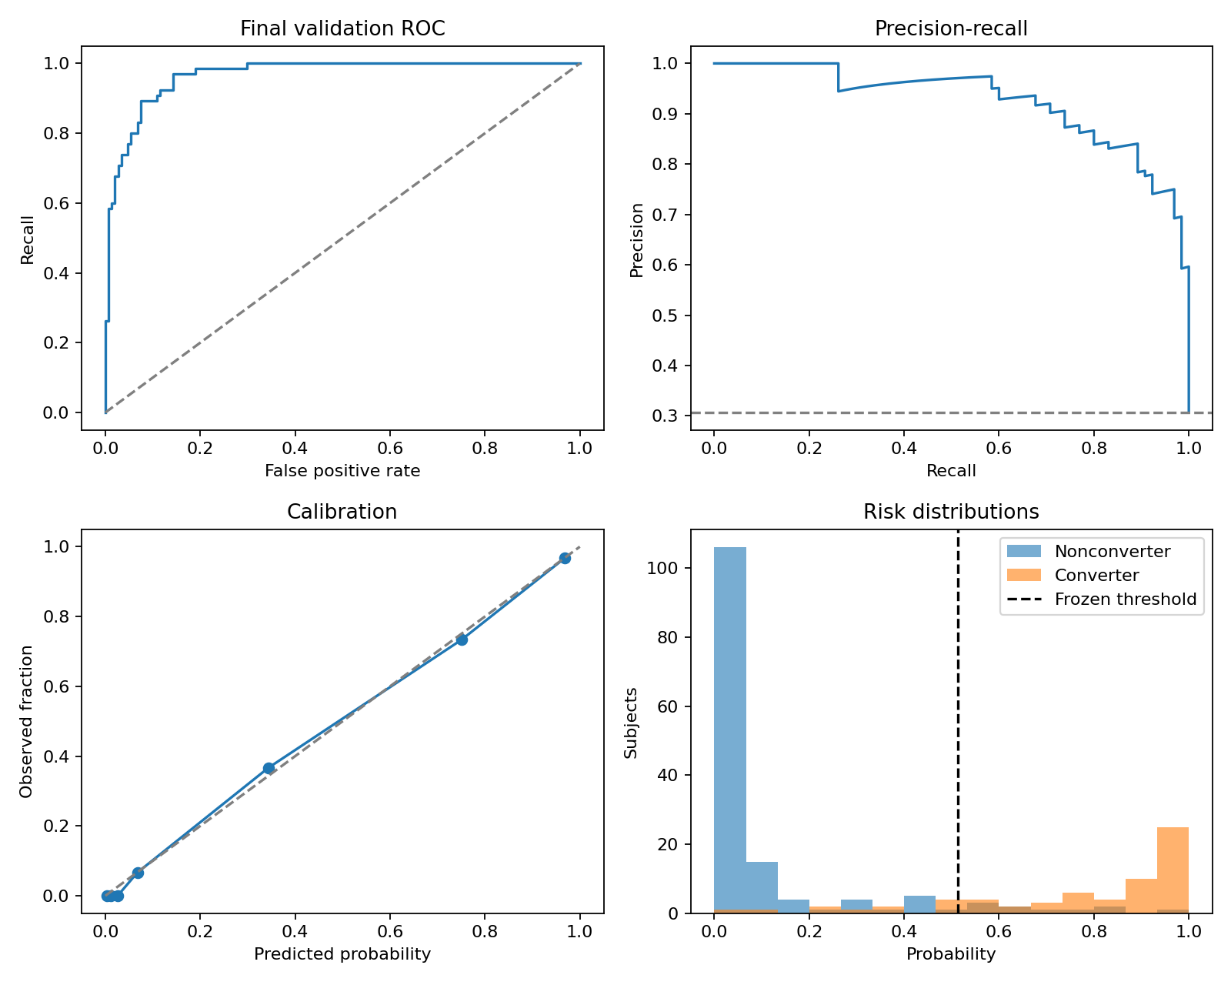
\includegraphics[width=.73\linewidth,height=.63\textheight,keepaspectratio]{figures/validation.png}
\par\smallskip\refstepcounter{figure}\small Figure \thefigure: Held-out performance of the shared frozen project predictor: ROC, precision--recall, calibration and risk distributions.\end{minipage}\par\medskip
The ROC curve lies close to the upper-left corner, indicating that the model can distinguish between dementia converters and non-converters across different classification thresholds. This observation is consistent with the ROC-AUC of 0.9667 obtained on the validation set. The Precision--Recall curve shows that the model maintains high precision over a wide range of recall values, although precision decreases as recall approaches 1.0.

The calibration plot shows the relationship between the predicted probabilities and the actual fraction of dementia converters. A curve closer to the diagonal reference line indicates better agreement between predicted and observed probabilities. The probability distribution plot shows that non-converters are generally concentrated towards lower predicted probabilities, whereas converters tend to have higher predicted probabilities. However, some overlap remains between the two groups, explaining why the model still produces false-positive and false-negative predictions.

\subsection{Confusion matrix}
\begingroup\small\renewcommand{\arraystretch}{1.16}
\begin{longtable}{@{}>{\raggedright\arraybackslash}p{0.29\linewidth}>{\raggedright\arraybackslash}p{0.32\linewidth}>{\raggedright\arraybackslash}p{0.33\linewidth}@{}}
\caption{Confusion matrix for the frozen project predictor on 212 validation participants}\\
\toprule \textbf{Actual class} & \textbf{Predicted non-converter} & \textbf{Predicted converter}\\\midrule\endfirsthead
\toprule \textbf{Actual class} & \textbf{Predicted non-converter} & \textbf{Predicted converter}\\\midrule\endhead
\midrule\endfoot\bottomrule\endlastfoot
Non-converter & 136 (true negative) & 11 (false positive)\\
Converter & 11 (false negative) & 54 (true positive)\\
\end{longtable}\endgroup
The model correctly identified 54 of the 65 observed converters and 136 of the 147 observed non-converters. It produced 11 false positives and 11 false negatives. The equal number of false positives and false negatives is why precision and recall have the same point estimate in this particular validation set.

\subsection{Development comparisons for the assigned models}
The tables report the best recorded mean development scores for the model families covered in this report. These are selected cross-validation results, not held-out test results.

\begingroup\small\renewcommand{\arraystretch}{1.16}
\begin{longtable}{@{}>{\raggedright\arraybackslash}p{0.45\linewidth}>{\raggedright\arraybackslash}p{0.24\linewidth}>{\raggedright\arraybackslash}p{0.24\linewidth}@{}}
\caption{Best recorded mean development F1 by model and panel}\\
\toprule \textbf{Feature panel} & \textbf{CatBoost} & \textbf{Random Forest}\\\midrule\endfirsthead
\toprule \textbf{Feature panel} & \textbf{CatBoost} & \textbf{Random Forest}\\\midrule\endhead
\midrule\endfoot\bottomrule\endlastfoot
Clinical (14 features) & 0.7968 & 0.8069\\
Core (28 features) & 0.8505 & 0.8397\\
Expanded (60 features) & 0.8448 & 0.8322\\
\end{longtable}\endgroup
\begingroup\small\renewcommand{\arraystretch}{1.16}
\begin{longtable}{@{}>{\raggedright\arraybackslash}p{0.33\linewidth}>{\raggedright\arraybackslash}p{0.105\linewidth}>{\raggedright\arraybackslash}p{0.105\linewidth}>{\raggedright\arraybackslash}p{0.12\linewidth}>{\raggedright\arraybackslash}p{0.1\linewidth}>{\raggedright\arraybackslash}p{0.12\linewidth}@{}}
\caption{Development scores for the strongest configuration of each assigned model}\\
\toprule \textbf{Model and strongest panel} & \textbf{Mean F1} & \textbf{Fold SD} & \textbf{Precision} & \textbf{Recall} & \textbf{ROC AUC}\\\midrule\endfirsthead
\toprule \textbf{Model and strongest panel} & \textbf{Mean F1} & \textbf{Fold SD} & \textbf{Precision} & \textbf{Recall} & \textbf{ROC AUC}\\\midrule\endhead
\midrule\endfoot\bottomrule\endlastfoot
CatBoost / core & 0.8505 & 0.0561 & 0.8077 & 0.9022 & 0.9613\\
Random Forest / core & 0.8397 & 0.0397 & 0.8373 & 0.8457 & 0.9618\\
\end{longtable}\endgroup
The core panel provided a strong balance of information and dimensionality. Adding more variables did not consistently improve performance. The expanded panel includes additional self-report and neuropsychological measurements, but it can also introduce more missing values and correlated information.

\subsection{Interpreting the tree model comparison}
Moving from the clinical to the core panel raised mean development F1 for both models. Adding the expanded candidates did not raise the best recorded F1 for either tree model. Core CatBoost had greater mean recall than core Random Forest (0.9022 versus 0.8457), while the forest had greater mean precision (0.8373 versus 0.8077). This comparison describes an operating tradeoff on development folds; it does not identify causal features or establish a significant difference.

The saved experiments do not provide a tree-specific feature importance or final validation confusion matrix. A tree feature-attribution analysis would need its own fitted estimator and evaluation protocol. No coefficient plot from the shared frozen predictor is attributed to the tree models.

\section{Discussion}
The validation results indicate that the selected baseline model can distinguish observed five-year dementia converters from non-converters within the labeled ADNI cohort. The ROC-AUC of 0.9667 indicates strong ranking performance on this particular held-out set. The precision and recall values of 83.08\% show that the chosen threshold achieved a similar balance between false-positive and false-negative classifications.

However, accuracy should not be interpreted alone. A simple model that predicts every validation participant as a non-converter would achieve 69.34\% accuracy because non-converters are the majority class, but it would identify none of the 65 converters. The higher accuracy of the selected model is therefore more meaningful when considered together with recall, specificity, F1-score and ROC-AUC.

The core panel gave the highest recorded F1 for both tree families covered here. Their development scores help compare settings, while the shared final validation describes a separately frozen predictor. Extra features may bring additional missingness and correlation.

A subgroup result requires particular care: all 65 validation converters belonged to the MCI subgroup. The validation CN/SMC subgroup contained 87 participants but no converters, so sensitivity and positive-class discrimination for that subgroup cannot be estimated from this split. The overall performance must therefore not be presented as evidence that the model has been validated for cognitively normal participants.

The literature paper provides a complementary direction. Its attention model learns interactions among brain regions from rs-fMRI connectivity matrices, whereas our model uses numerical clinical and biomarker variables. The two approaches demonstrate different ways of learning from ADNI data, but a direct comparison would require the same participants, prediction target, split strategy and evaluation protocol.

\section{Conclusion}
This BTP developed a baseline-only machine-learning pipeline to predict observed dementia diagnosis within five years using ADNI tabular data. The project involved reviewing multiple ADNI tables, selecting baseline-eligible features, constructing outcomes from longitudinal diagnosis records, handling missing values and comparing several classification algorithms. Particular attention was given to preventing temporal leakage and keeping the final validation participants separate from model fitting and threshold selection.

The strongest tree candidate was CatBoost on the core panel, with mean development F1 of 0.8505 versus 0.8397 for the strongest Random Forest. These scores are separate from the shared frozen predictor's held-out accuracy of 89.62\%, precision and recall of 83.08\%, and ROC AUC of 0.9667. Further validation is needed before clinical use.

\section{Limitations and Further Work}
\subsection{Limitations}
Incomplete follow-up: 698 baseline participants did not have enough observation to establish a five-year negative outcome. Excluding these participants may create selection bias because follow-up availability can be related to health, survival, study phase or visit attendance.

Uncertain acquisition dates for some merged fields: baseline suffixes and source provenance were used, but exact acquisition timestamps were not available for every assay or image-derived composite.

Missing data may be informative: KNN imputation preserves participants with incomplete features, but it cannot guarantee unbiased estimates when biomarker availability is related to participant characteristics or health status.

Limited subgroup evidence: there were no converters in the validation CN/SMC subgroup, so the model's ability to identify future converters among cognitively normal participants cannot be assessed from this evaluation.

Outcome is not AD-specific: the target is harmonized dementia diagnosis in general, not a confirmed Alzheimer's disease etiology.

Tree-model evidence is limited to the recorded development comparisons. Independent tree-model calibration and individual-level feature-attribution plots were not produced.

\subsection{Further work}
Evaluate the frozen model on an independent temporal or external cohort, with enough CN/SMC converters to assess performance in early and preclinical groups.

Develop a survival-analysis version that can use participants with incomplete follow-up. This should account for right-censoring, diagnosis intervals and competing risks such as death, and should report time-dependent discrimination and calibration.

Reassess plasma biomarkers using a clearly defined pre-baseline sample window and compare feature panels on matched participants so that differences are not driven by cohort composition.

Study explanation stability across folds and cohorts with carefully designed feature-attribution methods. Explanations should not be interpreted as causal evidence.

Assess clinical usefulness through decision-curve analysis and operating thresholds selected with clinical input, before considering any user-facing risk interface.

The experiment records and implementation are available in the project repository \cite{project}. The archived split and fitted artifact support reproduction; patient data, individual predictions and model binaries remain local. The supplemental comparisons in these reports were recovered from saved development records without retraining or retuning the frozen predictor.

\clearpage
\begin{thebibliography}{9}\addcontentsline{toc}{section}{References}
\bibitem{pathak} H. Pathak, G. Reddy N, M. Acharya, and M. Mahadevappa, \emph{An Attention-Based Framework for Alzheimer's Disease Classification Using Resting-State fMRI}, 2026. \url{https://arxiv.org/abs/2607.26746}.
\bibitem{collection} Alzheimer's Disease Neuroimaging Initiative, \emph{Data Collection}. \url{https://adni.loni.usc.edu/quick-start-guide-asset/datacollection.html}.
\bibitem{docs} Alzheimer's Disease Neuroimaging Initiative, \emph{ADNI Documentation}. \url{https://adni.loni.usc.edu/help-faqs/adni-documentation/}.
\bibitem{forest} L. Breiman, \emph{Random Forests}, Machine Learning 45, pp. 5--32, 2001. \url{https://doi.org/10.1023/A:1010933404324}.
\bibitem{cat} L. Prokhorenkova et al., \emph{CatBoost: unbiased boosting with categorical features}, NeurIPS, 2018. \url{https://arxiv.org/abs/1706.09516}.
\bibitem{project} BTP project repository and frozen aggregate experiment records. \url{https://github.com/soumil-kumar/adni-dementia-prediction}.
\end{thebibliography}
\end{document}
